\subsection{Bildegjenkjenning}

Kongsberg gruppen la klare retningslinjer om at OpenCV skulle benyttes. I tillegg oppfordret Kongsberg gruppen til å implementere programvaren i programmeringsspråket Matlab, ettersom de internt bruker Matlab til prototyping. 

I prosjektets begynnende fase var siste stabile utgivelse av OpenCV versjon 2.4.8, som ikke var støttet programmering i Matlab. For å bruke Matlab og OpenCV sammen gjensto det da to alternativer. Versjon 3.0 av OpenCV, som var under utvikling, støttet Matlab. I tillegg fantes det et tredjeparts kompatibilitetslag, \emph{mexopencv}, som gjorde det mulig å programmere med OpenCV i Matlab. Begge muligheter ble undersøkt. \emph{mexopencv} skapte problemer ved kompileringen på med de ulike kombinasjonene av operativsystemene, og de ulike Matlab-versjon som gruppen hadde inne allerede. Videre hadde \emph{mexopencv} problemer med grafikkortene som ble benyttet på de ulike maskinene, som ikke var støttet. Utviklingsversjonen av OpenCV, på sin side, ville overhodet ikke kompilere. Antakelig skyldes dette at kodebasen for denne versjonen var under rask utvikling og dermed ustabil.

Etter å ikke ha fått Matlab og OpenCV til å fungere sammen, ble det valgt å gå for en løsning der Matlab implementerte programvaren for bildegjenkjenning i C++. Som konsekvens av å ha skiftet språk til C++, hadde utviklingen raskt fremtog. 
\subsubsection{Innhenting av bilde og konvertering}

Kameraet fremga et bilde i fargespekteret RGB\footnote{Red, Green, Blue}, som er lite egnet til å separere ulike farger fra hverandre. Valget ble dermed å heller benytte fargespekteret HSV\footnote{Hue, Saturation, Value}, som er hyppig brukt innen bildeprosessering. Hver bilde ble konvert i videoen fra RGB, som vist i figur [\ref{fig:firstiterationrgb}], til HSV, som vist i figur [\ref{fig:firstiterationhsv}], før bildene ble prosessert videre.

\begin{figure}[!ht]
	\centering
	\subcaptionbox{RGB\label{fig:firstiterationrgb}}
	{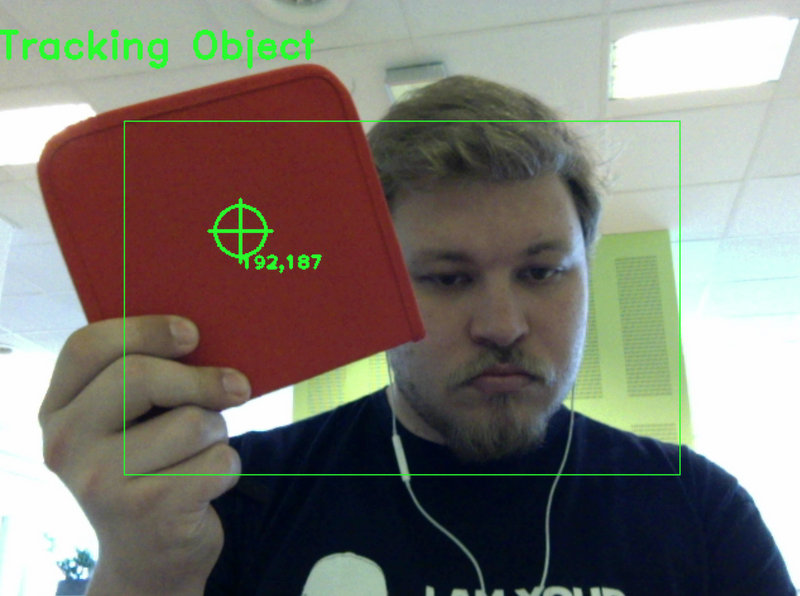
\includegraphics[width=0.45\textwidth]{img/first-rgb.jpg}}
	\subcaptionbox{HSV\label{fig:firstiterationhsv}}
	{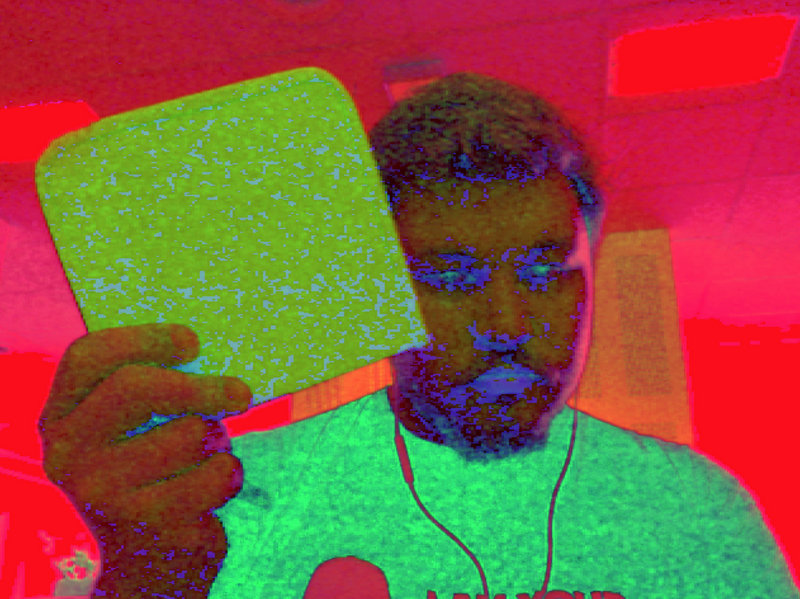
\includegraphics[width=0.45\textwidth]{img/first-hsv.jpg}}
	\caption{Bilde fra kamera i RGB og HSV}
\end{figure}

HSV baserer seg ikke på blanding av ulike farger, som RGB, men bruker nyanse, metningsgrad og lysverdi til å definere hver farge. Ved å konvertere bildet fra RGB til HSV forenkler dette jobben med å peke ut en spesifikk farge, samt forenkling av å skille objekter fra andre. Et eksempel på et problem ved å bruke RGB er at dersom et objekt blir flyttet fra lys til skygge, endrer ikke RGB-verdiene seg langs én akse, men derimot på både R-, G- og B-aksene på en måte som er vanskelig å forutse. HSV oppfører seg mer forutsigbart -- i dette eksempelet endrer fargeverdien seg hovedsakelig i V-aksen. \colorbox{yellow}{Dette lukter litt teori?}

\subsubsection{Deteksjon}

\begin{wrapfigure}[12]{r}{0.25\textwidth}
	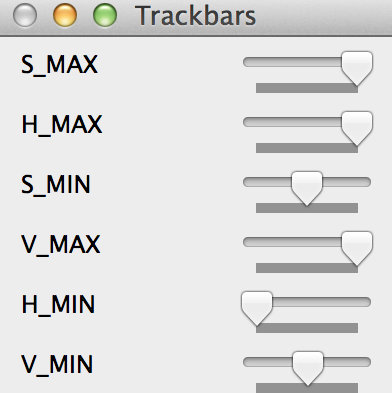
\includegraphics[width=\linewidth]{img/sliders.jpg}
	\caption{Slidere for å velge HSV-verdier}
	\label{fig:sliders}
\end{wrapfigure}

Etter å ha konvertert bildet til HSV, ble bildematrisen behandlet med et filter, som manuelt ble stillt inn med maksimum- og minimumverdier for \emph{hue}, \emph{saturation} og \emph{value}, som vist i figur [\ref{fig:sliders}]. Resultatet av dette var et binært bilde, der fargene som lå mellom disse maksimums- og minimumsverdiene er gjengitt i hvitt, mens alle andre farger er gjengitt i svart, som vist i figur [\ref{fig:firstiterationbinary}].

Ved at et binært bilde var prosessert, var neste steg å velge ut ett objekt fra bildet slik at det kunne spores. Definisjonen av objekt menes her et sammenhengende hvitt område i det binære bildet. Den algoritmen som ble skrevet valgte ut det største objektet, og returnerte objektets midtpunkt. Dersom det var for mye støy i bildet, det vil si for mange ulike objekter, returnerte algoritmen at objektet ikke ble funnet.

\subsubsection{Smoothing}

Objektet ble i det første steget fanget opp, men som presentert i figur [\ref{fig:firstiterationbinary}] er det mye støy i bildet. En smoothingalgoritme ble derfor implementert, noe som gikk over det binære bildet og fjernet mindre ansamlinger med punkter og fremhevet de som var større. Dette førte til et renere bilde, med færre og tydeligere objekter. Resultatet av smoothingen er presentert i figur [\ref{fig:seconditerationbinary}].

\begin{figure}[!ht]
	\centering
	\subcaptionbox{Før smoothing\label{fig:firstiterationbinary}}
	{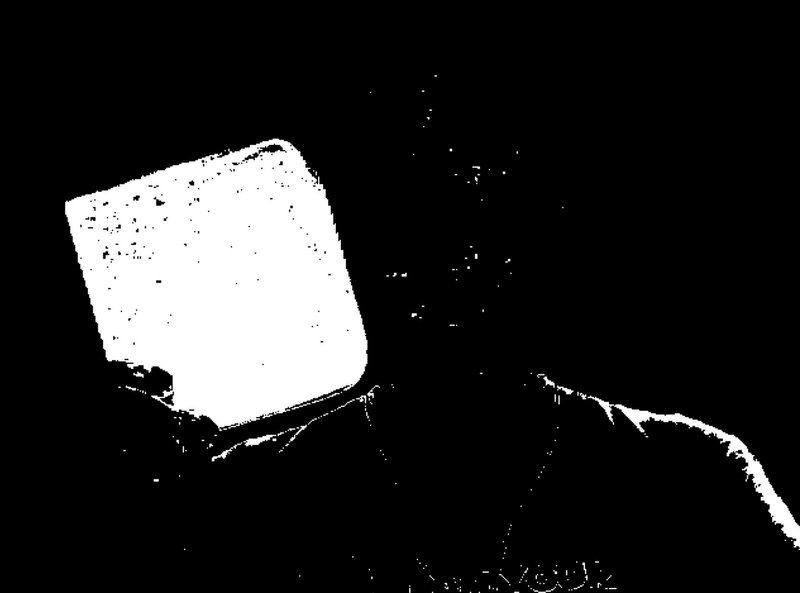
\includegraphics[width=0.45\textwidth]{img/first-binary.jpg}}
	\subcaptionbox{Etter smoothing\label{fig:seconditerationbinary}}
	{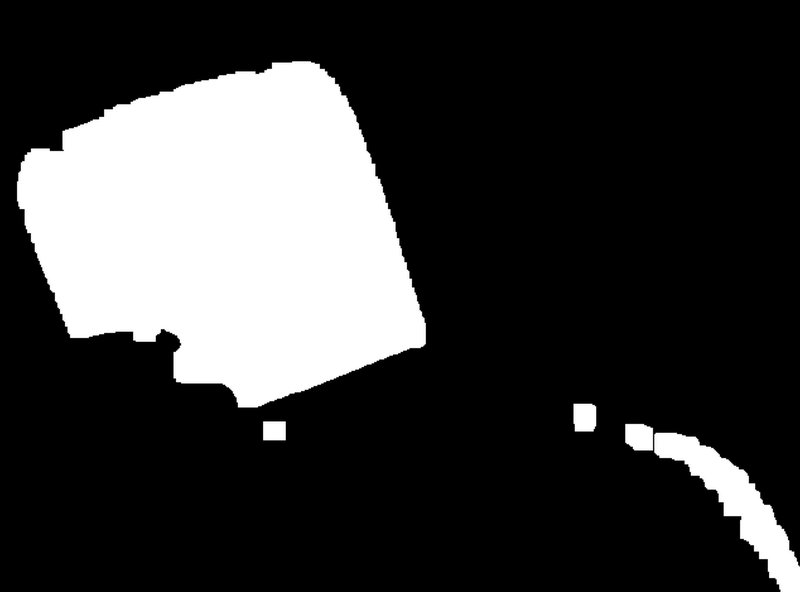
\includegraphics[width=0.45\textwidth]{img/second-binary.jpg}}
	\caption{Resultatet av filtrering av bilde før og etter smoothing}
\end{figure}

Smoothingen fremhevet de store objektene i bildet. Dette gjorde det betydelig lettere å fange opp kun det objektet vi var ute etter å følge, gitt riktig innstilling av fargefilterne, fordi små objekter i bildet med samme farge som objektet vi ville følge ble fjernet.

\subsubsection{Brukergrensesnitt}
\begin{wrapfigure}[12]{r}{0.3\textwidth}
	\centering
	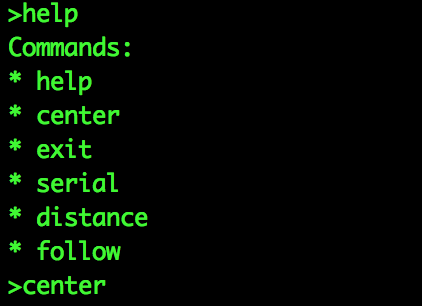
\includegraphics[width=\linewidth]{img/command-menu.png}
	\caption{En oversikt over de tilgjengelige kommandoene i kommandolinjegrensesnittet}
	\label{fig:commandmenu}
\end{wrapfigure}
Bestemmelsen av fargene i objektet ble automatisert ved at det ble implementert et enkelt kommandolinjegrensesnitt, der ved hjelp av kommandoen \texttt{center} kunne en be programmet om å følge etter fargen som befant seg i sentrum av bildet. Grensesnittet er vist i figur [\ref{fig:commandmenu}]. Kommandolinjegrensesnittet ble oppdatert ved utvidelse av nye funksjoner til programmet. 

For å gjøre det enklere å følge spesifikke objekter i kamerabildet, ble det implementert en funksjon som lot oss klikke på objekter i bildet for å følge dem. Både denne funksjonaliteten og \texttt{center}-kommandoen fungerte slik at fargeverdien til punktet som var i sentrum av bildet eller som ble klikket på ble hentet inn, og at sliderne automatisk ble satt til denne verdien pluss og minus en margverdi. Gode margverdier ble funnet eksperimentelt, og det ble bestemt at en marg på mellom $20$ og $30$ for hver av aksene \emph{hue}, \emph{saturation} og \emph{value} fungerte godt.

\subsection{Valg av hardware}

Det ble først bestemt at Arduino Uno skulle brukes til formålet. Fordelen var at det finnes et standard bibliotek for servoer for Arduino. I utgangspunktet skulle systemet ha et gyrometer som skulle måle orienteringen av riggen og kompensere for dette. På denne måten kunne kameraet stå vinkelrett uansett hvordan flyet bevegde seg. Det ble valgt å benytte seg av en modifisert utgave av biblioteket for MPU-6050 \cite{GyroLib}. Dette viste seg å bli et problem da Arduino ikke støtter multithreading. Det ble konflikt mellom PWM-delen av servobiblioteket og $I^2C$ som gyrometeret benytter seg av.

For å løse dette, ble det gjort forsøk på å benytte seg av to arduinoer. Lesingen av gyrometeret og pådrag til servoene skulle bli gjort på ulike arduinoer, med UART som kommunikasjonsprotokoll mellom dem. Erfaringene viste at arduinoen som skulle motta kommandoer mottok mye støy. Pådraget til servoene ble dermed veldig ustabilt.

Det ble da besluttet å gå over til Raspberry Pi. Som presisert i seksjon [\ref{sec:Pi}], har Raspberry Pi mulighet for multithreading. En lignende konflikt mellom PWM og I2C vil dermed ikke skje. Det oppstod imidlertid utfordringer da Raspberry Pi kun har 1 PWM-port. Det finnes en rekke biblioteker som løser dette ved å genere PWM-signal i programvaren og sende dem gjennom en vanlig digital port. Til dette formålet ble biblioteket WiringPi \cite{WirPi} benyttet. For gyrometeret ble et standard I2C-bibliotek brukt. Det viste seg at konfigurasjonen av WiringPi-biblioteket var tidkrevende, og det ble bestemt å gå tilbake til Arduino, men uten gyrometer.

Denne implementasjonen består av en Arduino som kjører servobiblioteket. Arduinoen får input fra en PC via USB, og gir pådrag til servoene basert på denne. Testene viste at servoene nå hadde en stabil oppførsel, og valget falt derfor på denne implementasjonen.

\subsection{Konstruksjon av riggen}

\subsubsection{Planlegging}
Riggens oppgave er å endre synsretningen til kameraet etter kommando fra bildegjennkjenningsprogramvaren. Synsvinkelen kan modeleres som en vektor, hvor retningen til vektoren er variabel. Hvis vektoren, $\bf{v}$, settes inn i et koordinatsystem med utspring i origo og sfæriske koordinater, kan situasjonen beskrives som i figur [\ref{fig:spher}].

\begin{figure}[h!]
	\centering
	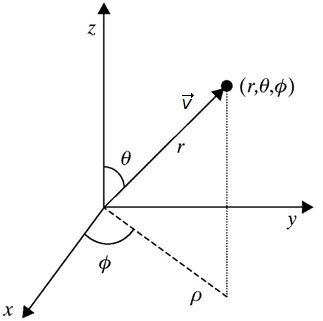
\includegraphics[scale=0.5]{img/RettVek.jpg}
	\caption{Sfærisk koordinatsystem}
	\label{fig:spher}
\end{figure}

Her er $\phi$ vinkelen mellom x- og y-aksene og $\theta$ er vinkelen mellom z-aksen og xy-planet. Siden riggen skal festes til et fly og kameraet skal se ned på bakken vil det ikke være behov for vinkelretningen å bevege seg inn i den øvre halvdelen av koordinatsystemet. Det betyr at $\phi$ og $\theta$ kun trenger 180 graders utslag for å dekke hele den nedre halvdelen. Dermed kan hele dette omerådet dekkes ved hjelp av to servomotorer med 180 graders utslag, satt sammen som illustrert i figur [\ref{fig:IdeRigg}].

\begin{figure}[h!]
	\centering
	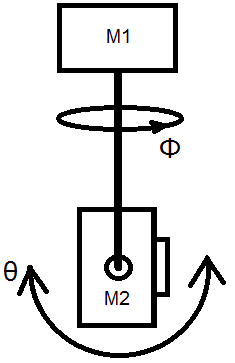
\includegraphics[scale=0.5]{img/BasicRiggIde.png}
	\caption{Servostyring av $\theta$ og $\phi$}
	\label{fig:IdeRigg}
\end{figure}

Kameraet festes til servomotor 2, som beveger seg i retning $\theta$. Samtidig beveger servomotor 1 på servo 2 og kamera i retning $\phi$. For å kunne trekke riggen inn i flyet ved landing ble det bestemt å feste riggen på en bom som kunne heves å senkes ved hjelp av ytterligere en servomotor, som vist i figur [\ref{fig:bom}].

\begin{figure}[h!]
	\centering
	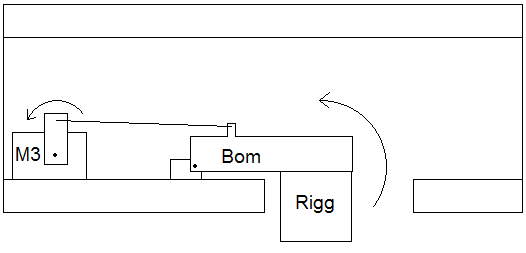
\includegraphics[scale=0.5]{img/Motor3.png}
	\caption{Servomotor 3 kan heve riggen inn i flykroppen.}
	\label{fig:bom}
\end{figure}

\subsubsection{Sammenstilling}

Riggen ble sammenstilt med målene på Kongsbergs prototypefly som utgangspunkt \cite{LocalHawkPDF}. Med disse målene ble det klart at servomotorene måtte være små i størrelse og valget falt på servomotoren HD-1600A. Med sine beskjedene fysiske mål på 21.3x11.6x22.8 mm og en vekt på $6$ g \cite{PowerHD}, ble HD-1600A ansett som perfekt for dette formålet. HS-50 fra Hitec ble også vurdert, men med lavere dreiemoment og betydelig høyere pris ble HD-1600A regnet som et bedre alternativ. For å bygge delene som skulle koble servoene sammen ble det brukt $6$ mm MDF-plater fordi disse er stive og relativt sterke. Dette fører til at de ikke bøyes eller gir etter ved raske rotasjoner. Figur [\ref{fig:RiggTegn}] viser hvordan servomotorene er koblet sammen og figur [\ref{fig:RiggBilde}] viser et bilde av den ferdige prototyperiggen. 

\begin{figure}[h!]
	\centering
	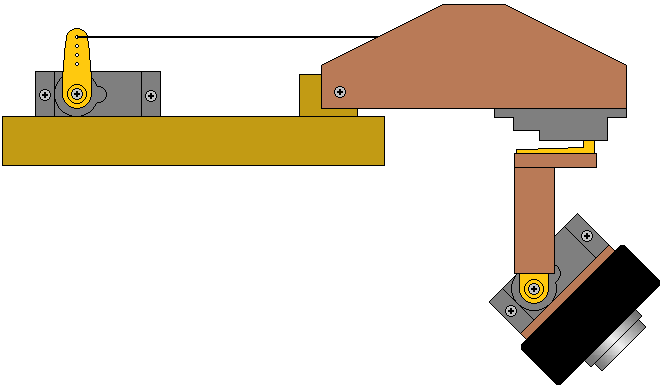
\includegraphics[scale=0.5]{img/RIGG_sattsammen.png}
	\caption{Tegning av mekaniske rigg}
	\label{fig:RiggTegn}
\end{figure}

\begin{figure}[h!]
	\centering
	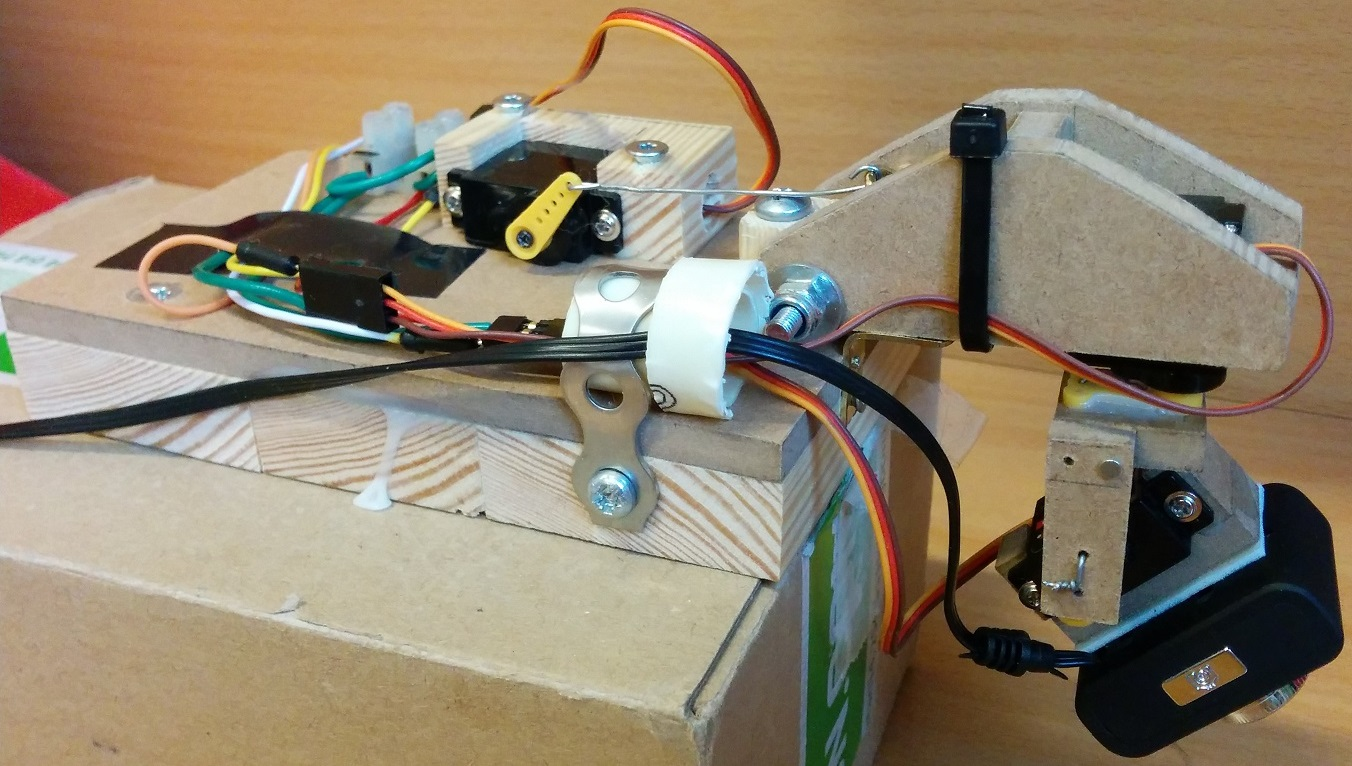
\includegraphics[scale=0.25]{img/Rigg_Bilde.jpg}
	\caption{Prototyperigg}
	\label{fig:RiggBilde}
\end{figure}

Servomotorene styres av et PWM-signal som genereres av en Arduino UNO. Biblioteket \texttt{Servo.lib} brukes for å kontrollere servoene gjennom tre I/O porter. Servo 1 er koblet til port 9, servo 2 er koblet til port 6 og servo 3 er koblet til port 3. Ved målinger viste det seg at hver servo kan trekke opp mot 250mA under last. Det ble valgt å bruke en ekstern 6V batteripakke med fire seriekoblede 1.5V AA batterier, koblet inn som vist i figur [\ref{fig:ArduSkjem}], i stedet for å la servoene trekke forsyningsstrøm rett fra $5$ V-pinnen til arduinokortet. Arduinokortet bruker strøm fra USB, som ikke kan levere mer enn $500$ mA på grunn av en innebygget sikring i kortet. Dermed kan ikke arduinokortet levere de ca. $750$ mA som trengs når alle servoene går med stor last samtidig.

\begin{figure}[h!]
	\centering
	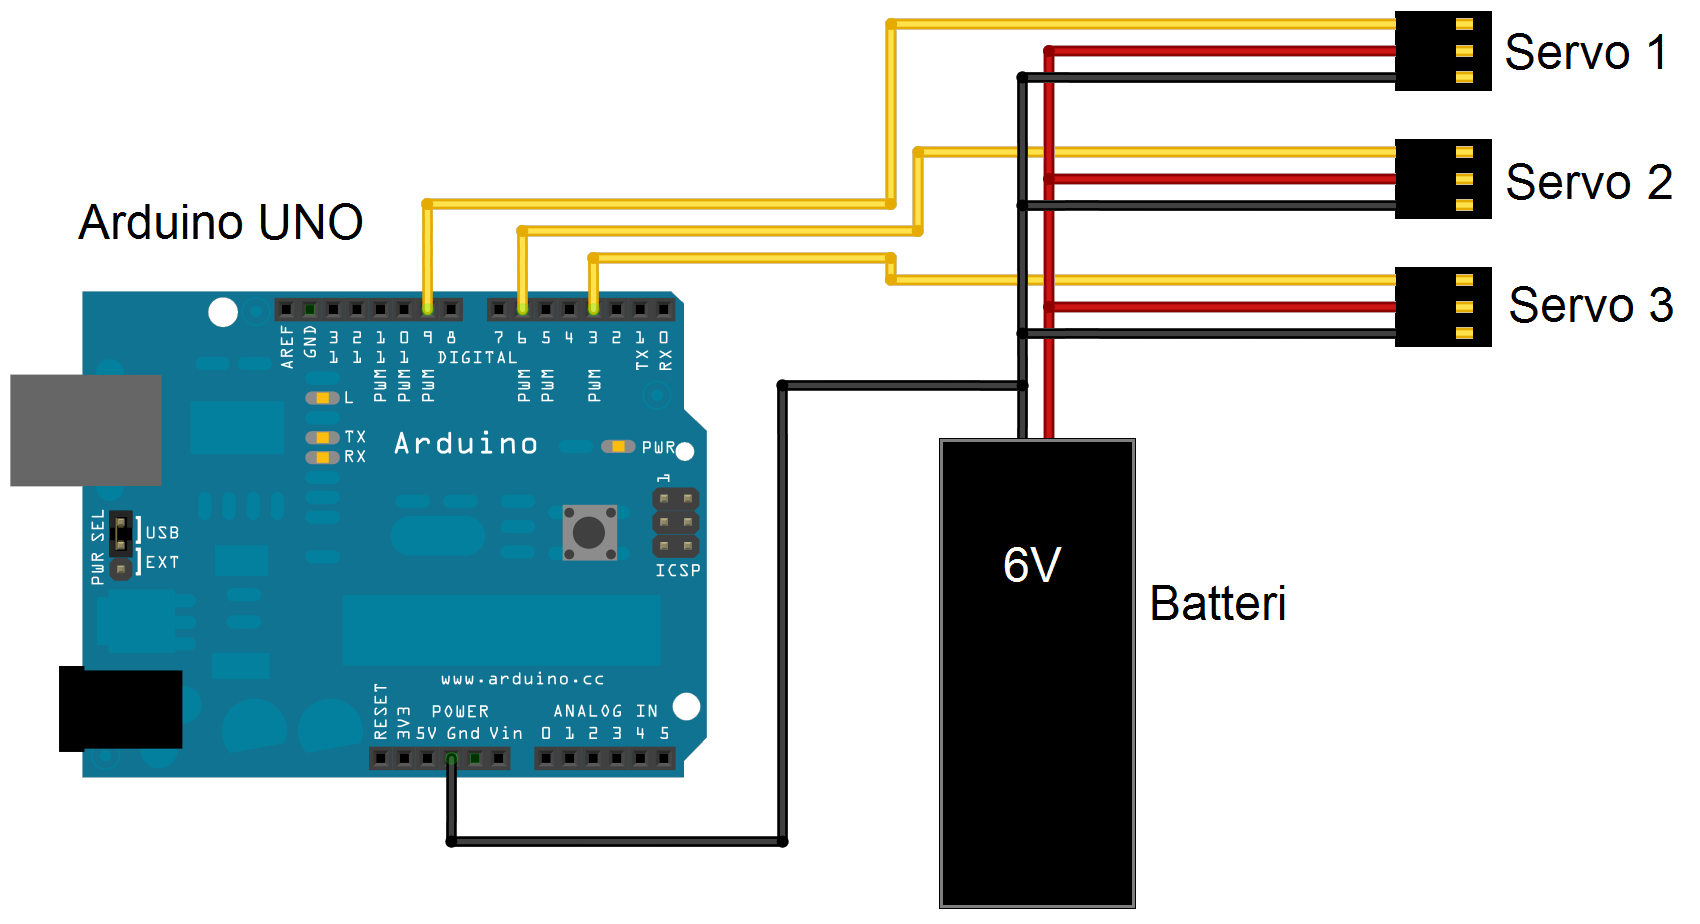
\includegraphics[scale=0.25]{img/KoblingsskjemaArduino.png}
	\caption{Koblingsskjema for Arduino}
	\label{fig:ArduSkjem}
\end{figure}  

Kommandoer sendes til Arduino via USB-porten. Kommandoer kan sendes som \texttt{Char} på formen \texttt{100a120b40c}, hvor tallene foran \texttt{c} forteller posisjon til servo 1, tallene for \texttt{b} gir posisjon til servo 2 og tallene foran \texttt{c} posisjonenen til servo 3. Dermed vil strengen \texttt{100a120b40c} flytte servo 1 til 100 grader, servo 2 til 120 grader og servo 3 til 40 grader. De gyldige vinklene er fra 0 til 180 grader. Hvis \texttt{200a} sendes vil servo 1 stoppe på 180 grader. 

\subsection{Styring av rigg}

På dette steget av arbeidet var det blitt ferdigstilt en rigg med et kamera som kunne styres med signaler fra en PC, og programvare som kunne detektere et objekt i bildet fra kameraet basert på fargen. For å koble disse to delene sammen, var det nødvendig med en metode for å oversette objektets posisjon i bildet til vinkelkommandoer som kunne sendes til riggen, med mål om å få kameraet til å peke direkte på det detekterte objektet.

Som tidligere beskrevet var den opprinnelige planen å kun bruke to av servomotorene til å styre kameraet, og bruke den tredje kun til å trekke kameraet inn i flyet. Det ble imidlertid klart at det var svært utfordrende å regne ut relasjonen mellom objektets posisjon i bildet og riggens bevegelse dersom disse to servomotorene ble benyttet. Som en enklere løsning ble det valgt å bruke servomotor 1 og 3 til å følge objektet. Med riktig forhåndsinnstilling av servomotor 2 står bevegelsesaksene til servomotor 1 og 3 omtrent normalt på hverandre, slik at de henholdsvis beveger seg langs tenkte x- og y-akser.

Fra kameraleverandøren ble det innhentet informasjon om størrelsen på kameraets synsfelt. Kombinert med det detekterte objektets avstand fra bildesenteret i piksler, ble det mulig å regne ut antall grader riggen måtte bevege seg for å plassere objektet i sentrum av bildet. Ved å til dette tallet legge til riggens nåværende posisjon, som ble lagret hver gang riggen ble bedt om å flytte på seg, ble en absolutt posisjon som riggen skulle flytte seg til regnet ut.

Det siste steget var å sende bevegelseskommandoene til Arduino-kortet, som kontrollerte servoene. Opprinnelig ble riggen bedt om å etter hvert nytt bilde fra kamera bevege seg hele avstanden i grader mellom sentrum av bildet og objektet. Dette førte til svært stor ustabilitet og oscillasjoner rundt de detekterte objektene. Dette ble løst ved å sette en begrensning på bevegelsen, der riggen aldri ble tillatt å bevege seg mer enn 2 eller 1 grad om gangen, avhengig av hvor nært objektet var sentrum av bildet.

Det ble senere oppdaget at punktet OpenCV beregnet som midten av det detekterte objektet gjerne varierte tilfeldig selv om objektet sto i ro, noe som førte til unødvendige bevegelser av riggen. Det ble dermed spesifisert i koden at dersom objektet var under 3 grader under sentrum, skulle riggen ikke bevege seg. En annen ting som ble bemerket var at motorene ikke opererte perfekt innenfor hele området $0$ til $180$ grader. Servomotor 1 hadde et ideelt bevegelsesområde på omtrent $15$ til $175$ grader, mens servomotor 3 kunne bevege seg mellom rundt $10$ og $140$ grader uten problemer. En sperre ble implentert som gjorde at dersom det var nødvendig for motorene å bevege seg utenfor disse intervallene for å følge et objekt, ble bevegelsene ikke gjennomført. Med disse begrensningene på riggens bevegelse på plass, fungerte objektfølgingen tilfredsstillende, uten for mye ustabilitet og med grei fart.